\section{Discussion and Conclusion}\label{sec:conclusion}

We have measured the local PNG parameter $\fnl$ using the scale-dependent bias in the angular clustering of LRGs selected from the DESI Legacy Imaging Survey DR9. Our sample includes more than $12$ million LRG targets covering around $14,000$ square degrees in the redshift range of $0.2< z < 1.35$. We leverage early spectroscopy during DESI Survey Validation \citep{desi2023sv} to infer the redshift distribution of our sample (Figure \ref{fig:nz}). \mr{Our power spectrum model accounts for various theoretical and observational effects such as RSD, magnification bias, survey geometry, and integral constraint. Most importantly, we utilize a novel machine learning-method to mitigate the effect of imaging systematics and reduce excess clustering power at low $\ell$.} 
In our fiducial analysis, \mr{which includes non-linear treatment using nine maps (Galactic extinction, stellar density, depth in $grzW1$, and psfsize in $grz$), we obtain $\fnl = 34^{+24(+50)}_{-44(-73)}$ with $p=1$ and $s=0.945$. The signature of local PNG is very sensitive to excess clustering power caused by imaging systematic effects. We have applied a series of robustness tests to investigate the impact of how the galaxy selection function is determined. Specifically, both linear and nonlinear methods are applied using various combinations of imaging systematic maps (including two external maps for the neutral hydrogen column density and photometric calibration error in the z band). We also examine the effect of different survey masks based on imaging properties and survey completeness. Overall, we find no change in the analysis that shifts the maximum likelihood value of $\fnl$ to a significantly different value (Figure \ref{fig:mcmc_dr9reg}, Figure \ref{fig:mcmc_dr9elmin}, and Table \ref{tab:dr9method}). The fiducial measurement \mr{(i.e., $-39<\fnl<84$} at 95\% confidence) is consistent with recent CMB and LSS measurements, as visualized in Figure \ref{fig:fnlhist}, and the findings are robust against $p$ and $s$ (Figure \ref{fig:fnl_magbias}).}

\begin{figure}
    \centering
    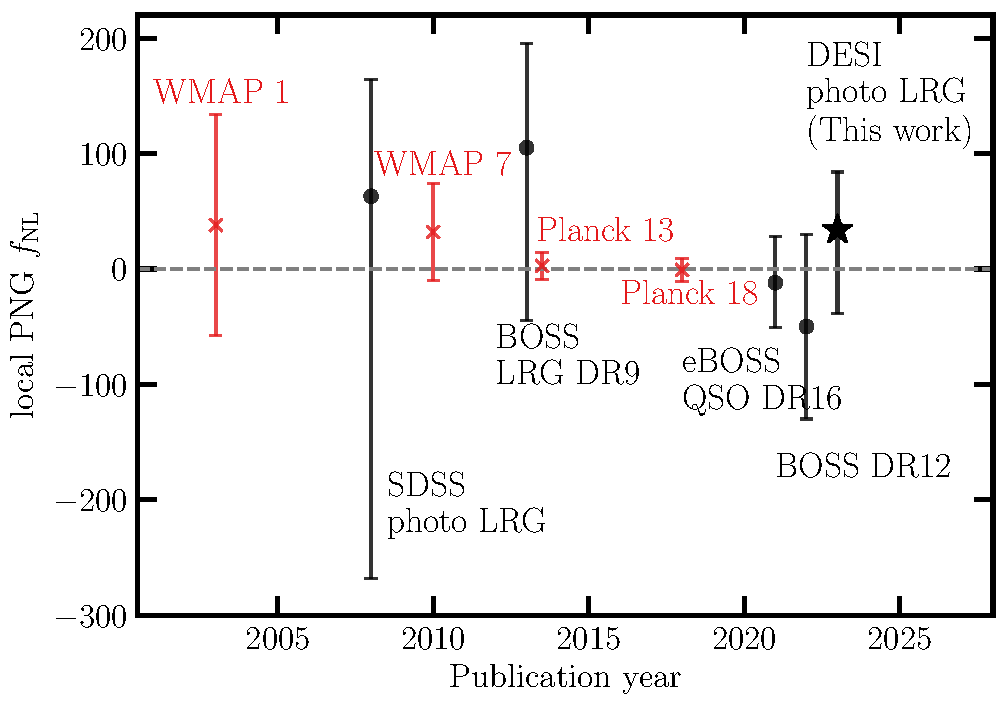
\includegraphics[width=0.45\textwidth]{figures/fnl_history.pdf}
    \caption{History of constraints on local PNG $\fnl$ at $95\%$ confidence from single-tracer LSS \citep{slosar2008constraints,2013MNRAS.428.1116R, mueller2022primordial, 2022PhRvD.106d3506C}, including our analysis with $\mr{-39}<\fnl<\mr{84}$ (DESI photo LRG) and CMB surveys \citep{Komatsu_2003, Komatsu_2010, planck13, akrami2019planck}. The median $\fnl$ value is used in case the maximum likelihood estimate was not reported in the reference.}
    \label{fig:fnlhist}
\end{figure}

\mr{As an attempt to identify the optimal approach for the treatment of imaging systematics, we conduct statistical tests based on the mean galaxy density and cross-correlations of the LRG density with imaging maps (Appendix \ref{sec:systests}). These tests reveal a preference for artificially diminishing the constraining power of the dataset, as we consistently remove excess clustering signal until $\fnl=0$ is recovered. While accounting for over-correction allows for the recovery of the removed signal, it comes at the cost of losing constraining power due to the removal of large-scale clustering information. Hence, there is a strong motivation for exploring alternative approaches to enhance the science yield of datasets in future studies of local primordial non-Gaussianity.}

\mr{With the aforementioned caveat in mind, Galactic extinction, depth in z, and psfsize in r are identified as the primary sources of systematics. The non-linear method with three maps is able most of the trends against all available templates. Using nonlinear three maps, we obtain a maximum likelihood value of \mr{$\fnl=46$} with a significant probability that $\fnl$ is greater than zero, $P(\fnl>0)=99.9$. Without accounting for the over-correction, the probability reduces slightly to $P(\fnl>0)=99.5$ per cent. The linear methods also yield constraints that are in tension with CMB ($P(\fnl>0)=99.9$). While we have not calibrated the over-correction for the linear cases, it would only make the result more significantly non-zero and we cannot envision this changing any of our conclusions. With nonlinear three maps, either we have measured an $\fnl$ signal that is inconsistent with CMB measurements or there is a hidden source of systematic contamination in our sample which cannot be mitigated with only three maps. It is noteworthy that there is a body of exciting work in the literature exploring models where $\fnl$ (or another non-Gaussianity parameter) varies with scales and evades the CMB constraint while showing up in the LSS \citep{2008JCAP...04..014L,sefusatti_2009, becker_2011, Becker_2012}. For instance, \cite{Becker_2012} presents forecasts on $\fnl(k)$ from the Planck bispectrum and DES power spectrum assuming the power-law model of scale-dependent non-Gaussianity, and illustrate the differences in the sensitivity of CMB and LSS probes to $\fnl$ on various scales. Thus, in principle, CMB and LSS can measure different $\fnl$ values, but whether and what kind of specific scale dependent $\fnl$ model would be consistent with our measurement and the CMB measurement would require detailed work.} 

Our analysis can be considered as the first attempt to identify major systematics in DESI, so we can be ready for constraining $\fnl$ with DESI spectroscopy. Internal DESI tests of the photometric calibration were unable to uncover DESI-specific issues, e.g., when comparing to Gaia data. The most significant trends that we find are with the E(B-V) map. The source of such a trend would be a mis-calibration of the E(B-V) map itself or the coefficients applied to obtain Galactic extinction corrected photometry. Such a mis-calibration would plausibly be proportional in amplitude to the estimated E(B-V) map, though it may not have E(B-V)’s spatial distribution. In order to explain the $\fnl$ signal we measure, such an effect would need to be approximately twice that of the trend we find with E(B-V). There are ongoing efforts within DESI to obtain improved Galactic extinction information, which will help establish if this is indeed the cause. \mr{Additionally, cross-correlations of the DESI LRG density with the CMB lensing map is more stable in terms of systematics and can complement the results presented in this work. We can further improve the estimation of the galaxy survey selection function by combining our neural network-based method with forward-modeling techniques, such as Obiwon \citep{kong2020}, but we will leave that for future work.} 